\section{Discussion}
In the previous sections we have presented back-ground information on capacitive proximity sensors and various prototypes of this technology in different application domains within smart environments. In the following section we are building on the collected information to perform a meta-analysis of the acquired data, discussing benefits and limitations of the technology, compare it to competing technologies and give some guidelines to parties interested in developing further applications in this domain. 
\subsection{Limitations}
\begin{table}[htbp]
  \centering
  \caption{Overview of capacitive proximity sensing limitations}
    \begin{tabular}{p{4cm}p{6cm}}
    \toprule
    \textbf{Name} & \textbf{Examples} \\
    \midrule
    \textbf{Environmental influence} & Static electric fields, dynamic electric fields, temperature, humidity, conductive objects \\
    \textbf{Physical range} & Small differences in capacitance, reduction due to influences, physical limitations \\
    \textbf{Object detection} & Small number of data points, a priori knowledge \\
    \bottomrule
    \end{tabular}%
  \label{tab:cap_limitations}%
\end{table}%

Despite the potential that has been described in the previous sections there are various limitations of capacitive proximity sensing that we can put into the different groups of environmental influence, physical range and object detection that will be described in more detail in the following section. A short overview is given in Table \ref{tab:cap_limitations}.
\subsubsection{Environmental Influence}
One of the main limitations of capacitive proximity sensors is their sensitivity towards environmental influences. Any factor that modifies an electric field will also affect the measurement of a capacitive sensor. The current environmental parameters, like temperature and humidity are having a considerable effect on the atmosphere in which the electric field propagates. However, those changes are usually over a longer period of time and can be compensated using a factor for drift, as described in the previous sections about noise reduction. A more challenging factor is the other electric devices in the environment that emit stronger electromagnetic fields. While persistent sources, such as permanent electric installations can usually be countered using a galvanic isolation there are other non-obvious challenges. E.g. we noticed that certain plasma TVs are able to disturb the measurement and increase noise levels consider-ably. This change is even varying according to screen content. A minor effect is the presence of high-frequency fields that are getting more prevalent in modern IT equipped environments. Instead of the 2.4GHz and 5GHz ranges that are often used in wire-less communication, capacitive proximity sensors can operate in the range of a few kHz to one MHz. 
An additional issue might arise when placing sensors close to each other. The created electric fields may disturb the measurement if some electrodes are charged and create fields to adjacent electrodes while they are discharged for measurement. Consequently, specific charge-discharge cycles or multiplexing methods have to be used to counter this effect. 
A major challenge is dealing with conductive objects that are permanently placed in the immediate sensing environment. It is difficult to distinguish the object we want to detect from a disturbing object, if their influence on the electric field is similar. Long term data analysis may help in performing a successful detection.
The CapFloor prototype is affected by environmental influences the most, given the small size of the electrodes relative to the interaction area and the changing environment on top of the floor. We are using a strong noise reduction algorithm and drift compensation to create a more stable result while reducing the detection range.
\subsubsection{Physical Range}
\begin{figure}[h]
\centering
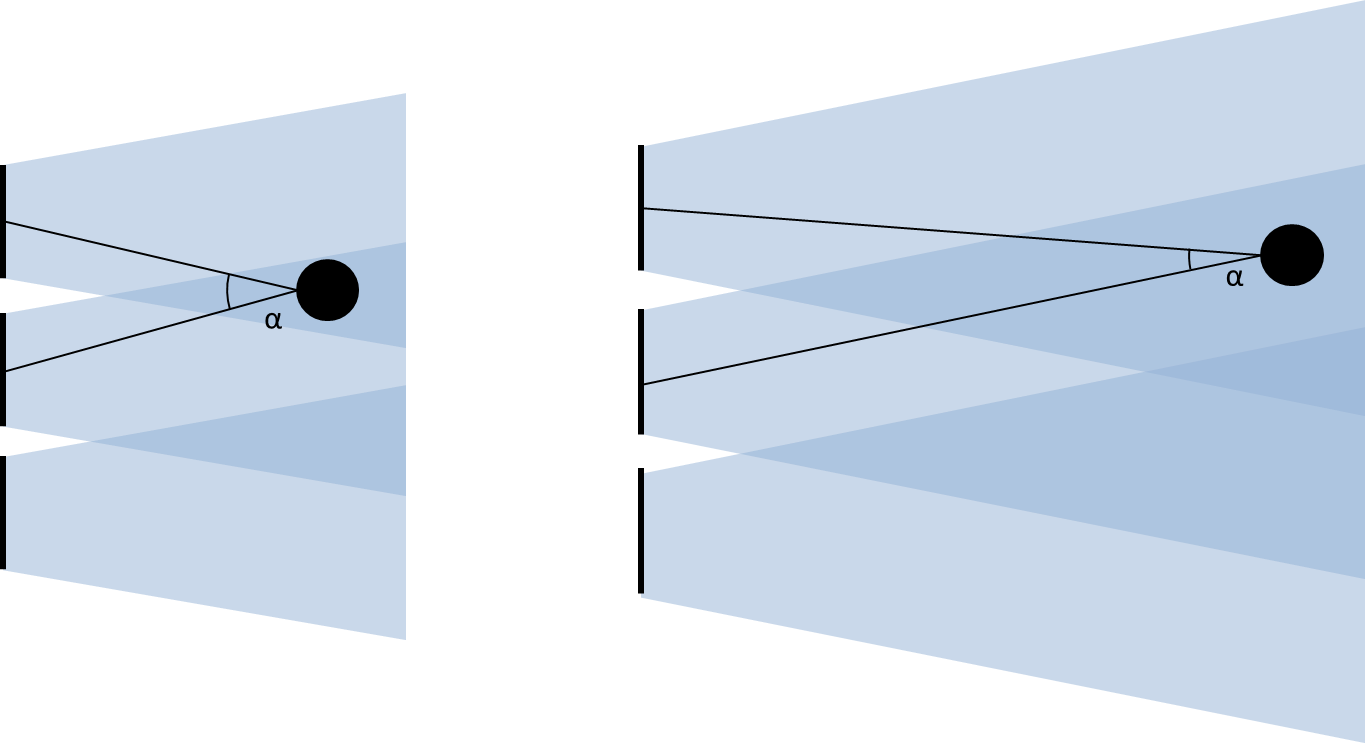
\includegraphics[width=0.6\textwidth]{images/limit_distance.png}
\caption{Reduced angular resolution on smaller, distant objects}
\label{fig:disc_ang_resolution}
\end{figure}
The physical range of the generated electric field is one of the main limiting factors of capacitive proximity sensing. In order to detect objects that are further away we have to increase the electric field strength sufficiently. This is easier the larger the electrode is, as its potential capacitance is higher. However, this also leads to distant objects having an ever smaller influence on the overall capacitance, and we need more precise measurement circuits and longer measurement times to improve the signal-to-noise ratio. Additionally, looking at smaller objects the angular resolution will decrease as shown in Figure \ref{fig:disc_ang_resolution}. This makes it more difficult to get a precise localization as the immanent noise leads to an angular error. While this can be compensated using more sensors, the far distance would require us to use large electrodes that have to be placed further apart resulting in a huge area that would have to be equipped with sensor electrodes.
In general the achievable resolution is not comparable to vision based system and has to be taken into consideration when designing the specific application. A balance between electrode size, physical range and achievable resolution has to be found.
The MagicBox size does not allow an integration of very large electrodes. Instead we are optimizing the available space in order to achieve a detection that lets us detect hands in a distance between 15 and 20 centimeters.
\subsubsection{Object Detection}
\begin{figure}[h]
\centering
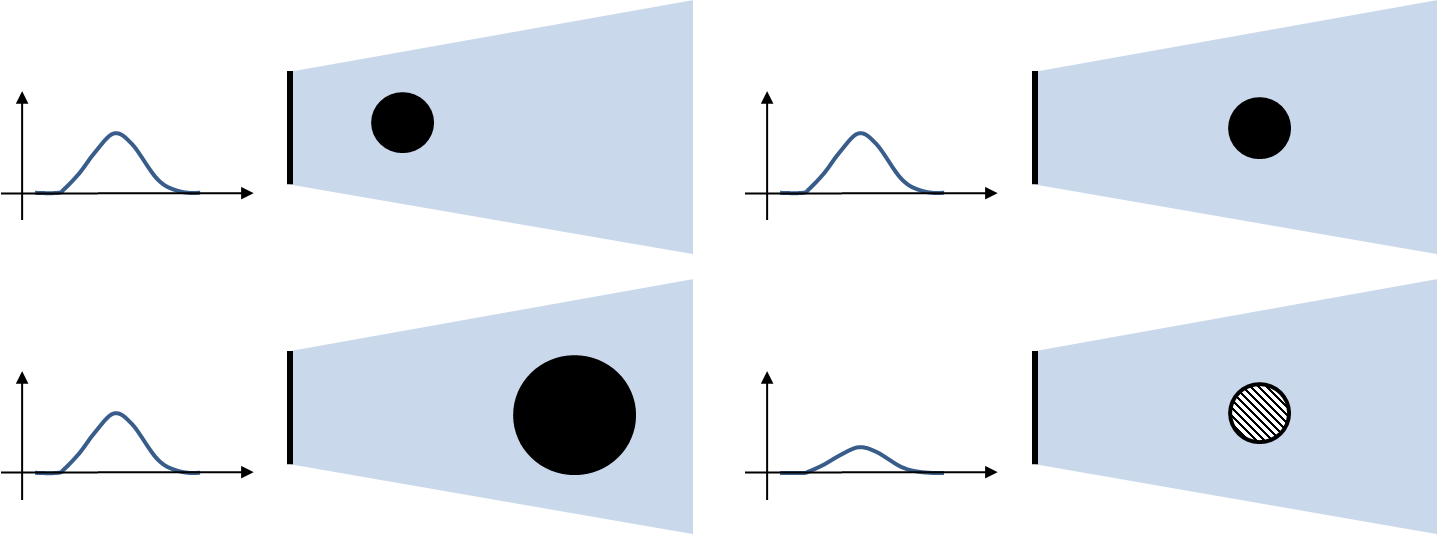
\includegraphics[width=0.6\textwidth]{images/limit_detection.png}
\caption{Same response to differently sized objects (left), different response to varying materials (right)}
\label{fig:disc_obj_detection}
\end{figure}
Object detection using capacitive sensors can be partially compared to object detection using camera systems, with a single sensor being equivalent to a single photo sensor. The light intensity measure is comparable to field intensity and likewise we can't distinguish if the measurement is caused by a weak source in close proximity or a strong source at a further distance. As a practical example the capacitive sensor can't decide if one hand is close to the sensor or two hands are a bit further away. This effect makes it challenging to provide object detection and we usually have to combine the information from various sensors to get a good idea about object shape and size. Due to the presented challenges in physical range and electrode size, capacitive proximity sensing systems do not have the same level of scalability as opposed to cameras, where millions of photo sensors can be placed in very small areas. 
Additionally, the effect of an object on the electric field is not always closely correlated to the object dimensions, but instead based on conductivity, material and other factors. We may get the same response to different objects at different distances or get a varying on similarly sized objects made of different materials, as shown in Figure \ref{fig:disc_obj_detection}. 
The Active Armrest has gestures for one and two fingers that are distinguished using a simple threshold. If another object is entering the field or the person has larger fingers the system will fail to properly differentiate gestures. Accordingly some other compensation methods should be used.
\subsection{Benefits}
\begin{table}[htbp]
  \centering
  \caption{Overview of capacitive proximity sensing benefits}
    \begin{tabular}{p{4cm}p{6cm}}
    \toprule
    \textbf{Name} & \textbf{Examples} \\
    \midrule
    \textbf{Versatility} & Flexible electrode design, scalability, different sensing methods \\
    \textbf{Unobtrusiveness} & Invisible application, non-disturbing frequency range \\
    \textbf{Processing Complexity} & Small number of sensors, variable dynamic range \\
    \bottomrule
    \end{tabular}%
  \label{tab:cap_benefits}%
\end{table}%

After discussing the various limitations of capacitive proximity sensing, the following section will give an overview of the benefits.  Similar to the previous section we have three groups, namely versatility, unobtrusiveness and processing complexity. Some examples within these groups are shown in Table 6.
\subsubsection{Versatility}
A main benefit of capacitive proximity sensing is the versatility in which they can be applied. The flexibility of electrode materials, size and geometry allows specifically creating highly individual applications. Example electrodes include transparent metal oxide layers, woven conductive thread, copper wires, PCB boards or simple aluminum foil. 
The sensors systems are also highly scalable. By choosing appropriate voltages and frequencies it is possible to add a high number of sensors to a single object. Using smart measurement windows and different multiplexing methods, sensors can be placed close together and electrodes may act as both sender and receiver.
The different sensing methods presented - loading mode, shunt mode and transmit mode enable a variety of different sensing patterns. The human body can be used as both sender and receiver and smart electrode layouts allow using a smaller number of processing units. 
In conclusion, it is possible to add capacitive sensing to most everyday objects to enable different forms of interaction, create natural interfaces and smart objects. Our prototypes are using different electrode materials, flexible or solid electrodes, conductive thread, wires, shielded or non-shielded layouts. 
\subsubsection{Unobtrusiveness}
 \begin{figure}[h]
\centering
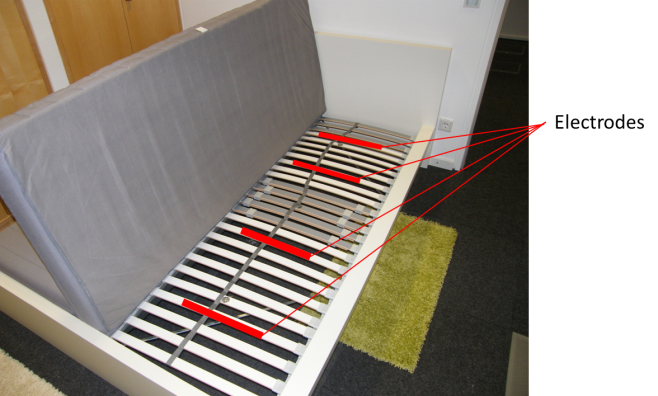
\includegraphics[width=0.6\textwidth]{images/disc_unob_bed.png}
\caption{Electrodes and sensors hidden below mattress of Smart Bed}
\label{fig:disc_unob_elec}
\end{figure}
Electric fields are not usually perceived by persons, unless they are of exceptional strength. Furthermore they propagate through many materials that we are typically using in our environment, including most plastics, wood or tiles. This allows us to invisibly apply capacitive proximity sensors without a strong effect on the measurement. Application below several centimeters of covering is possible, if the electrodes are designed properly for sensing in this distance.
The frequency range in which the sensors are operating is usually not in an interval that disturbs other electronic systems. Thus it is feasible to use capacitive sensing even in environments, where non-disturbance is a main requirement.  Additionally the used frequencies are not considered to be biologically active, and good results can be achieved using small currents. 
It is possible to equip most conductive objects directly with capacitive proximity sensors and hide them below non-conductive objects with minimal spatial requirements. Our Smart Bed and Active Armrest prototypes are using sensor sets that are completely invisible from the outside and communicate wirelessly to a PC only using a power supply. Figure \ref{fig:disc_unob_elec} shows the electrodes and sensors hidden below the mattress of the Smart Bed.
\subsubsection{Processing Complexity}
An appropriate analogy of capacitive proximity sensors is a single photodiode. As opposed to a light intensity we are measuring capacitance. While the information we can gain from such a measurement is limited, the processing required to analyze the signal is also low. Performing signal analysis on an array of 16 capacitive sensors is comparable to processing the image of a 4x4 pixel camera. Therefor it is easy to create highly integrated systems with very low-power devices for performing any subsequent data analysis. While it is possible and in many cases beneficial to use complex data processing algorithms for object detection it is in most cases still possible to replace them with simpler methods for a comparable result.
In many applications it is even viable to opt for a quantized capacitance measurement. In the case of a touch sensor a single binary measure is sufficient. However, it is also possible to select various different levels and reduce the dynamic range to an easily computable value that is 4 or 8 Bit long. Depending on the chosen algorithm this dynamic range reduction can occur either in pre-processing or high level processing.
With the exception of the Capacitive Chair our prototypes are using simple data processing methods that can be easily applied on embedded systems. A preferred method for object localization is the weighted average algorithm. Regarding model-based data processing, even very simple cylindrical models, such as the one used for the Smart Bed, are capable to reliably predict numerous postures that are relevant in real world applications. In general, the low requirements for data preprocessing, allows dedicating more resources to high level data processing algorithms if the specific application is resource con-strained. 
The OpenCapSense toolkit that is the base for most of our prototypes has a fairly powerful micro-controller that is able to implement all of the processing steps - thus enabling highly integrated, low-power capacitive proximity sensing prototypes that can be used in smart environment applications.
\subsection{Guidelines}
After discussing the limitations and benefits of capacitive proximity sensors, the final section of this chapter will give some general guidelines on their application. The first step of this process is a decision if capacitive sensors technology is suitable for the given application. This part should be driven by three questions.
What do I need to measure in my application scenario?
Capacitive proximity sensors can measure the presence and properties of conductive, grounded objects. This includes the various application scenarios shown in the previous sections. However, if the application requires measuring properties of unsupported objects that are non-conductive, a different technology should be chosen.


\textit{What sensing technologies are supporting the required measurements?}


It may be the case that multiple technologies sup-port the measurements required in this specific applications. Cameras often can provide similar recognition as capacitive sensors, e.g. in indoor localization applications. In this step all potential sensing technologies should be collected.
Are capacitive proximity sensors beneficial for my scenario?
An evaluation of the different candidates is the final step and should lead to a decision about the most suitable sensing technologies. If the distance is too high for capacitive proximity sensors or enough processing power is available and lighting conditions are static, cameras might be more suitable. This should be driven by the different benefits and limitations of  the technologies.
If there is a decision in favor of capacitive sensors the next step is to design the specific electrode layout. Similar to technology selection we can use a few basic questions to get an idea of what layout to use.


\textit{How many sensors are required to get the measurement?}


The number of sensors required is depending on the area we want to cover, the specific object parameters that have to be determined and the desired resolution. The electrodes are inherently limited in size, as a single sensor can only charge and discharge to a specific maximum capacity. Therefore, if a large area has to be covered more electrodes and sensors are necessary. If we just want to measure the presence of a hand a single electrode may suffice. If orientation and position are interesting we need to combine measurements from various sensors.


\textit{What should be the size and geometry of the electrodes?}


This is closely related to the previous question. If the application is not restricting the available space, the electrode should be approximately of the same size as the object that is to be detected. This generates the highest difference in capacitance when the distance is changing. 


\textit{What is the best electrode material to use?}


Copper is always a good first choice to create electrodes. If elasticity is necessary we can use copper foil and solid copper if that is of no concern. For transparent electrodes we will have to use one of the previously presented materials, such as ITO. If electrodes have to be integrated into cloth, conductive thread is a good candidate. Any conductive material will act as an electrode, thus the application and budget should be the primary driver of this decision.


\textit{Does my application require any shielding?}


Shielding allows detecting only objects approaching from a certain direction. If the application re-quires this additional hardware, because it is anticipated that other objects might disturb the measurement, shielding should be used.
Finally, if the hardware is designed as desired the different variations of data processing have to be chosen and configured according to the application.
Using baseline calibration is beneficial in the vast majority of applications. Having a distinct starting point simplifies all further steps of high-level data processing, such as normalization and setting different thresholds. This step may only be omitted in very stable environments and if the system has sufficient a priori information to operate on raw data. Drift compensation should be handled in a similar fashion. The common methods are not computationally expensive and having a stable baseline over time allows the same algorithms to be applied in a more robust fashion. The method and configuration of noise reduction are strongly depending on the specific case. Some form of noise reduction might be required in most applications. Yet, according to the type of noise different methods can be used. If outliers are an issue a median filter is appropriate; if a smoother signal is desired an average filter can be used. 
Regarding high-level data processing there are manifold variations of methods. Data-driven machine learning algorithms are a good method if we have a small set of potential outcomes of our applications, e.g. the different postures that could be recognized on a chair or couch. If our application has many different potential outcomes, e.g. the thousands of potential locations in a hand tracking system, it is typically beneficial to use a model-driven approach. However, these models may be supported by data-driven algorithms, such as particle filters. One example is the Swiss-Cheese object tracker by Grosse-Puppendahl et al. \cite{grosse2013swiss}. The data processing examples shown in the previous sections give an idea of the decision rationale in various application domains.
We can say in conclusion that capacitive proximity sensors are a viable, or even, ideal solution for a considerable number of different applications. However, a certain level of preparation is required in the design process to create a system that benefits from the technology.
